\documentclass[11pt]{article}
\usepackage[letterpaper, margin=1in]{geometry}
\usepackage[shortlabels]{enumitem}
\usepackage{amsmath}
\usepackage{graphicx}
\usepackage{setspace}
\usepackage{titling}
\usepackage{cite}
\usepackage{url}
\title{BVA Legal Semantic Modeling}
\author{Harout Boujakjian, Clara Buss, Ahn Hoang, Elizabeth Kenis, Tim Roger}


\setstretch{1.3}
\setlength{\droptitle}{-4em}

\begin{document}
\maketitle

\section*{Problem}

The Board of Veterans' Appeals (BVA) of the U.S. Department of Veterans Affairs has to read through tons of claims cases a day dealing with veterans who are appealing previous PTSD diagnosis decisions made by the VA board. The enitre process is done manually and it's not hard to imagine how a huge backlog of claims could pile up. The process of a veteran filing a disability claim and submitting it to BVA can take upwards of 125 days before the BVA issues a decision based on the submitted paperwork \cite{BVAaudit}. This is a process that certainly lends itself well to some form of automation. 

Identifying the patterns of factual reasoning using machine learning can provide a way to automate argument mining \cite{Walker2019AutomaticCO}. The data set used in this report provides the means begin this process. Additionally, supervised learning has not permeated the legal domain in the same that it has with other fields like genomics, image classification for handwritten digits, etc. It's interesting to see how well models can predict the classification of sentences extracted from these legal documents. Dr. Vern Walker, a professor of law at Hofstra University, has spent some of the past few years working on analyzing the complexity that exists in these legal documents \cite{Walker2017Semantic}. The approach to sentence classification that is taken in this paper could be extended to many types of legal cases (e.g. immigation cases, vaccine cases, etc.). Ultimately in this specific problem, the goal is to be able to submit a new case into the model and have it print out all of the predictions. Then, one can sift through the specific classification they desire, e.g. finding of fact sentences, and use it to readily put together a new report for an appeals case. This speeds up the process for the both the veterans' lawyers and the Board who can each use the tool separately. However, before all of this can take place, there needs to be an underlying model that will be able to accurately predict sentence classifications.

\section*{Understanding the Data}

The data set involves 20 actual decisions issued by BVA from 2013 to 2017\footnote{Full data set can be found at https://github.com/vernrwalker/VetClaims-JSON} \cite{LLTdata}. The cases are broken down into sentences and each of the sentences is labeled with one of six rhetorical roles: Finding of Fact Sentence, Reasoning Sentence, Evidence Sentence, Citation Sentence, Legal Rule Sentence, and Sentence. The last category, Sentence, is a catch-all label for anything that does not fall into the five other categories. The labeling of the sentences was conducted by Dr. Walker and the Law, Logic, and Technology Lab at Hofstra Univsitry. The data set contains 2,526 sentences in total. Each sentences is treated as one observation, which means there are 2,526 rows of data. It is important to emphasize that this is not a ``Big Data'' problem that is traditionally encountered in Natural Language Processing (NLP). Most NLP models require hundreds of thousands of rows of training data in order to produce accurate predictions. Here, we are trying to see how well we can classifiy sentences based on this relatively small data set (given today's standards).

The five rhetorical roles are defined below \cite{LLTdata}:

\begin{itemize}
\item[] \textbf{Finding Sentence}: A finding sentence is a sentence that primarily states an authoritative finding, conclusion or determination of the trier of fact – a decision made “as a matter of fact” instead of “as a matter of law.”
\item[] \textbf{Reasoning Sentence}: A reasoning sentence is a sentence that primarily reports the trier of fact’s reasoning based on the evidence, or evaluation of the probative value of the evidence, in making the findings of fact.
\item[] \textbf{Evidence Sentence}: An evidence sentence is a sentence that primarily states the content of the testimony of a witness, states the content of documents introduced into evidence, or describes other evidence.
\item[] \textbf{Legal Rule Sentence}: A legal-rule sentence is a sentence that primarily states one or more legal rules in the abstract, without stating whether the conditions of the rule(s) are satisfied in the case being decided.
\item[] \textbf{Citation Sentence}: A citation sentence is a sentence whose primary function is to reference legal authorities or other materials, and which usually contains standard notation that encodes useful information about the cited source.
\end{itemize}

The breakdown of total rhetorical roles will play an important part in predictions. The bar chart in Figure \ref{rrcount} below displays the counts of rhetorical roles. The most common rhetorical role among the data is evidence sentences. Besides evidence, the other roles show up in much smaller fractions. Given the count of evidence sentences, it's possible to hypothesize that the model may predict that rhetorical role more accurately than the others. It could also label sentences as evidence more frequently simply because evidence sentences have the highest count.


We can start to get an idea of what the most common words are in the corpus by tokenizing the sentences and counting the words. In Figure \ref{wordcount}, we notice that the words service, veteran, evidence, and PTSD are the top four most common words. In BVA appeals cases related to a veteran's condition following a war, this falls in line with what is expected. However, given how common these words are, it is very likely that they show up in many different sentences, regardless of the sentence's rhetorical role. This will become a problem when using classification models since the models need to be able to distinguish sentences from each other. Thus, we need to find a metric more suitable to this type of problem.

\begin{figure}[h]
  \centering
  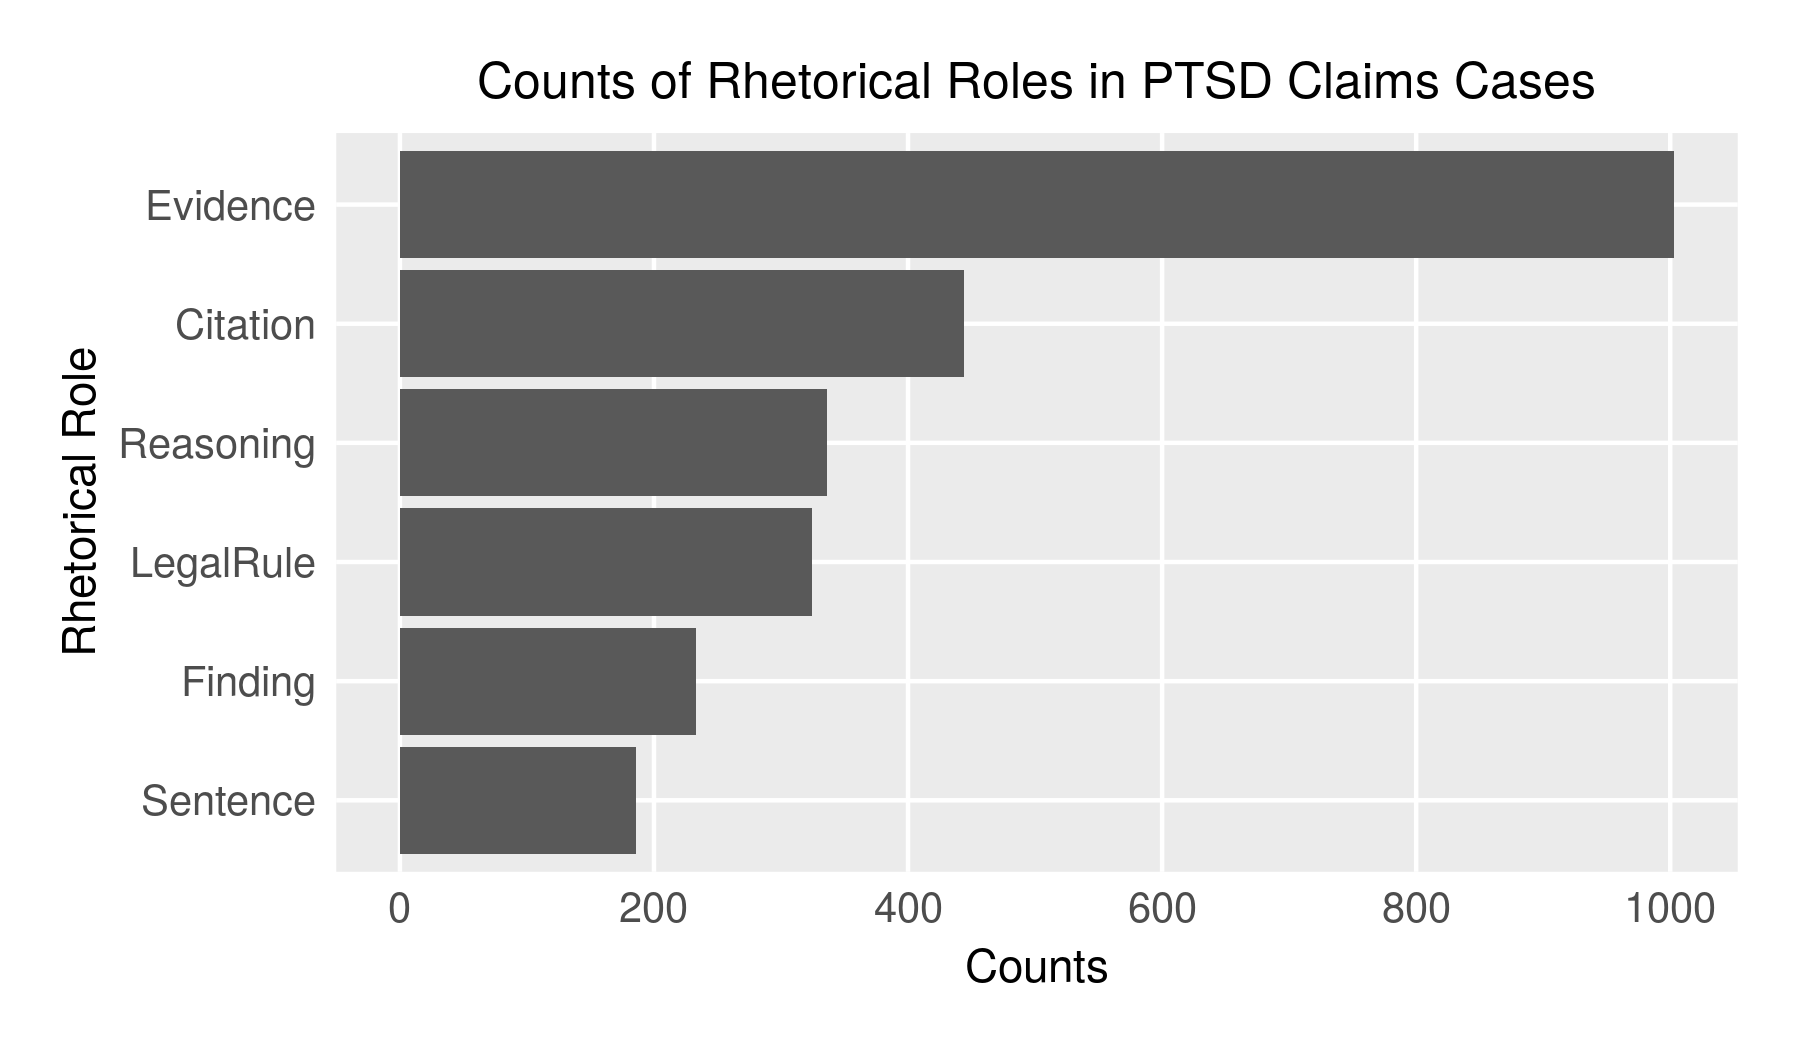
\includegraphics[scale=0.7]{images/barchart}
  \caption{Bar plot of rhetorical role counts}
  \label{rrcount}
\end{figure}

\begin{figure}[h]
  \centering
  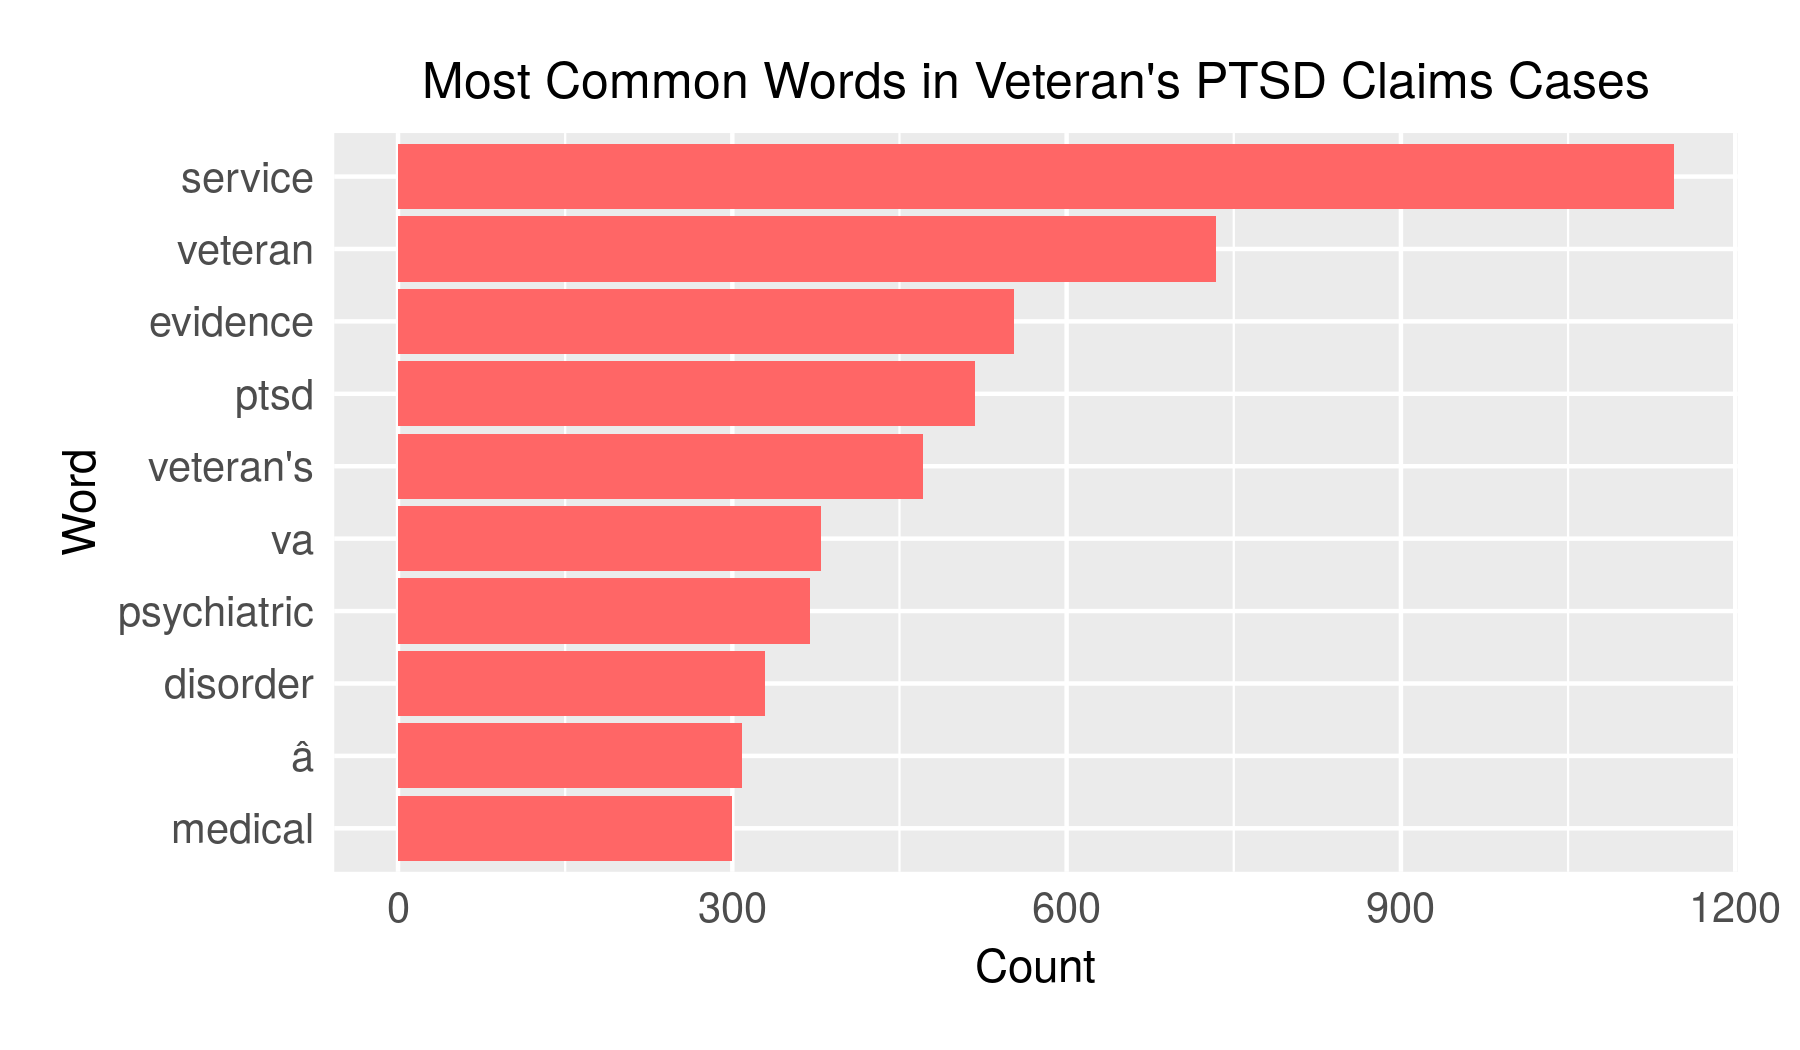
\includegraphics[scale=0.7]{images/word_count}
  \caption{Bar plot of word counts}
  \label{wordcount}
\end{figure}

In order to get an idea of what words may be the most important in each rhetorical role, we use the term frequency-inverse document frequency (tf-idf) statistic. This number is the product of the count of a word in all of the sentences (term frequency) and the inverse of how many sentences contain the word in total (inverse document frequency) \cite{christopherdmanning2008introduction}. Tf-idf is commonly used in NLP data exploration and modeling. The graph belows facets by rhetole role and displays the top 8 words with the highest tf-idf in each category. The tf-idf vectorization was done using the TfidfVectorizer in scikit-learn \cite{scikit-learn}.

\begin{figure}[h]
  \centering
  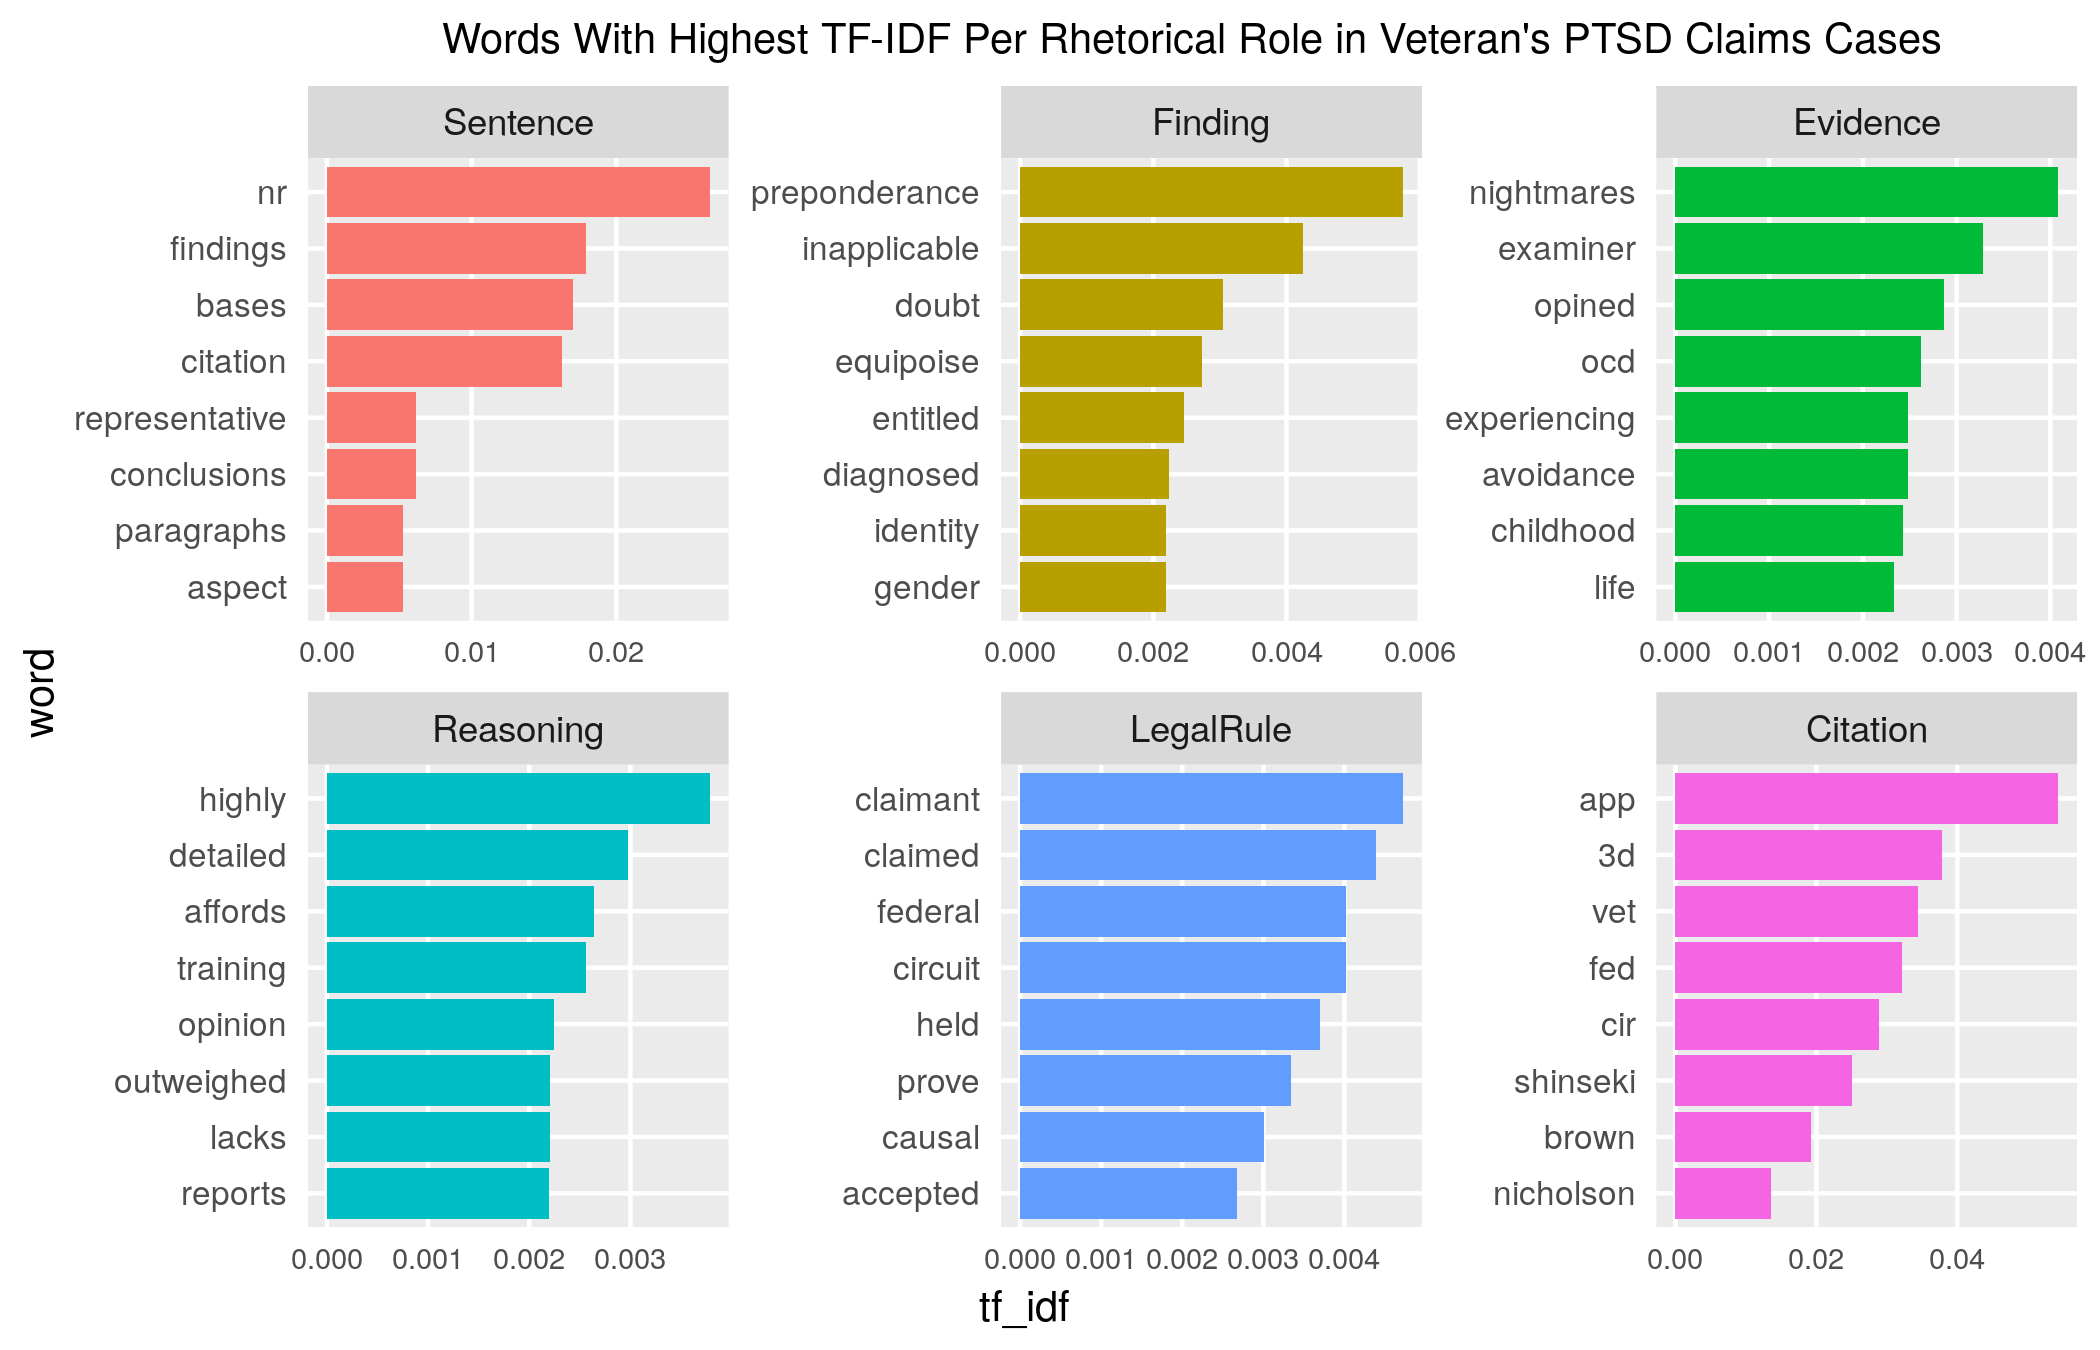
\includegraphics[scale=0.85]{images/facet_tf-idf1}
  \caption{Top 8 TF-IDF scores per rhetorical role}
  \label{tfidfcount}
\end{figure}

If we inspect the plot in Figure \ref{tfidfcount}, we notice some interesting words pop up in each of the respective categories. The actual tf-idf values can be hard to interpet, but relative to other words we may get an idea of the most important words. For evidence sentences, we see the words ``nightmares'', ``ocd'', ``experiencing'', ``avoidance'', ``childhood''. These are the kinds of words we would expect to see for evidence sentences (e.g. The veteran was experiencing nightmares about his childhood). In the legal rule category, we see ``claimant'', ``federal'', ``circuit'', ``causal'', and ``prove''. This is again expected with legal rule sentences, which generally describe abstract legal rules. Citation sentences appear to have somewhat uncommon words and this is precisely because they usually involve references to pages in law books, names of court cases, addresses, etc. In Sentences, we see ``finding'' and ``citation'', which may potentially be referring to headers. In contrast, it's hard to tell if the words in the Reasoning and Finding of fact rhetorical roles fit. They are generally more complex sentences than the other categories and the hardest to predict.

\section*{Models}

The main feature engineering invovled converting the dataframe of sentences and rhetorical roles to a tf-idf matrix. First, the sentences were tokenized into words and the counts of each word were saved. Next, the stop words (e.g. the, and, have, which, etc.) were dropped from the corpus of words. Then the tf-idf values were calculated for each of the words. Finally, the dataframe was cast into a matrix with each row being a sentence and each column indicating whether the specific word was included in the sentence and it's td-idf value. Thus every cell either contained a 0 if the word was not present in the sentence, or the respective tf-idf statistic if it was. This final matrix is highly sparse (with sparsity at 98\%).

Labeling of sentences is a categorical classification problem. For each of the models used, the data was split into a training, validation, and testing set with 70/10/20. The first model used was multinomial logstic regression from scikit-learn, which uses regularization by default \cite{scikit-learn}. Several values were tested for the regularization constant C: 1, 10, 50, 100, 1000, 2000. A value of $C=10$ was ultimately used as it had the highest accuracy on the validation set. The results of the model are in Tables \ref{table:LR} and \ref{table:prLR}. The average accuracy for all of the rhetorical roles is 82.61\%. Upon inspecting the table, citation sentences have the highest recall of 97\%. This is to be expected since citation sentences have lots of odd characters and words compared to the other five sentence types. The next highest recall score are evidence sentences with 92\% being predicted correctly. This also makes sense there are more evidence sentences than all other types, which was shown in Figure \ref{rrcount}. Interestingly, the precision was 87\%, which is not that bad. That means that the classifier was not predicting all sentences as evidence just because there were more in the training data set. In the case of finding of fact, legal rule and reasoning sentences, the predictions are in 60-70\%. This is not as great, and indicates that better text preprocessing and feature engineering may be necessary to improve performance. These sentences also have more complicated sentence structures than the rest.

\vspace{1.4em}
\begin{table}[h]
  \centering
  \begin{tabular}{| c| c| c| c| c| c| c|}
    \hline
    & \multicolumn{6}{|c|}{\textbf{Actual}} \\
    \hline
    \textbf{Predicted} & citation & evidence & finding & legal rule & reasoning & sentence \\
    \hline
    citation  & \textbf{89} &    6    &  0     &    2      &        1  &    0 \\ 
    evidence  &  1   & \textbf{183} &       2   &     9     &       13  &    2  \\
    finding   &    0   &    1    & \textbf{32}  &    1      &        5  &    5  \\
    legal rule &    2   &    1    &        0    & \textbf{42} &    2     &    3  \\
    reasoning &    0   &    7   &        8    &    13    &  \textbf{43} &   2  \\
    sentence  &    0   &   1    &        5     &    2   &         1     & \textbf{22}\\
    \hline
  \end{tabular}
  \caption{Confusion matrix for multinomial logistic regression}
  \label{table:LR}
\end{table}
\vspace{0.3em}

\vspace{1.4em}
\begin{table}
  \centering
  \begin{tabular}{| c | c | c | c | c |}
    \hline
    &                   precision  &   recall &  f1-score  &  support \\
    \hline
    citation sentence &       0.91 &     0.97 &     0.94 &       92 \\
    evidence sentence &       0.87 &     0.92 &     0.89 &      199 \\
    finding sentence &       0.73 &     0.68 &     0.70 &       47 \\
    legal rule sentence &       0.84 &     0.61 &     0.71 &       69 \\
    reasoning sentence &       0.59 &     0.66 &     0.62 &       65 \\
    sentence &       0.71 &     0.65 &     0.68 &       34 \\
    \hline
  \end{tabular}
  \caption{Precision/Recall table for multinomial logistic regression}
  \label{table:prLR}
\end{table}
\vspace{0.3em}


The second model tested was a simple neural network using tensorflow and keras in python \cite{tensorflow2015-whitepaper}. The architecture of the neural net included two dense layers with a dropout layer in between. The purpose of the dropout layer, with half of the nodes dropped, is to prevent overfitting. The first dense layer had 512 nodes with a ReLU (rectified linear unit) activation function and is a popular choice for the first layer. It is a simple activation function. The second dense layer had only 6 nodes and a softmax activation function. This is a multinomial version of a logistic regression and is necessary to produce the final vector of probabilites for each sentence. Lastly, the max of the vector of probilities is taken for each sentence and this is the prediction for the class. As with a lot of neural network architecture, the layers were put together using trial and error to determine what worked best. The reason for three layers as opposed to 10+ is to keep the neural network simple and see how well the results compare with the multinomial logistic regression. The number of epochs, an iteration over the whole x and y data provided, used was 8. The batch size, the number of samples used per gradient update, was 64 \cite{tensorflow2015-whitepaper}. The confusion matrix for the neural network is Table \ref{table:NN} and the precison/recall results is in Table \ref{table:prNN}.


\vspace{1.4em}
\begin{table}[h]
  \centering
  \begin{tabular}{| c| c| c| c| c| c| c|}
    \hline
    & \multicolumn{6}{|c|}{\textbf{Actual}} \\
    \hline
    \textbf{Predicted}  &  Citation & Evidence & Finding &LegalRule &  Reasoning & Sentence \\
    \hline
    Citation &        76 &     0 &    0 &      0 &        1 &   1  \\
    Evidence &        0 &   194 &    3 &      1 &        16&   3\\
    Finding &         0 &      3 &   29 &     0 &        5 &   4 \\
    Legal Rule &       1 &      1 &   1 &      59 &        1 &  1 \\
    Reasoning &       0 &      9 &  9 &        7 &      38 &   4  \\
    Sentence &        0 &      1 &  2 &        2 &       3 &  31 \\
    \hline
  \end{tabular}
  \caption{Confusion Matrix for Neural Network}
  \label{table:NN}
\end{table}
\vspace{0.3em}


\vspace{1.4em}
\begin{table}
  \centering
  \begin{tabular}{| c | c | c | c | c |}
    \hline
    &                   precision  &   recall &  f1-score  &  support \\
    \hline
    Citation Sentence &      0.97 &     0.99 &     0.98 &       77 \\
    Evidence Sentence &      0.89 &     0.93 &     0.91 &      208 \\
    Finding Sentence &      0.71 &     0.66 &     0.68 &       44 \\
    Legal Rule Sentence &       0.92 &     0.86 &     0.89 &       69 \\
    Reasoning Sentence &      0.57 &     0.59 &     0.58 &       64 \\
    Sentence &      0.79 &     0.70 &     0.75 &       44 \\
    \hline
  \end{tabular}
  \caption{Precision/Recall table for neural network}
  \label{table:prNN}
\end{table}
\vspace{0.3em}

The overall accuracy for the neural network is 83.53\%. Similar to the logistic regression model, the neural predicts citation sentences with the highest recall at 99\%, and evidence sentences at 93\%. But in this case Legal Rule sentences are predicted correctly at 86\%. This is in major contast to logistic regression, that was only able to predict them correctly $\sim$61\% of the time. The important takeaway here is that both models performed quite well with only approximately 2,500 sentences (even slightly less if the training/validation/testing split is considered) and the results were relatively decent and a strong starting point. This is an enticing result and is what led the team to focus on developing the product for now, and returning back to model performance at a later time.

\section*{Further Improvements}

There are certainly improvements that can be made to the model in the future. Adding more sentences to the training set will very likely increase the performance of the model. The LLT lab is in the process of labeling more cases, and they will used to train in model training in the future. The emphasis on this modeling effort still not being a big data problem will exist since there are only so many labels that the lab can generate. In terms of text preprocessing, there was not much done besides converting the words to lower case, removing stop words, and casting the data to a tf-idf matrix. More intelligent preprocessing of the text can also improve performance. This will especially be true in the case of finding of fact and reasoning sentences, since they have complex sentence structures. Additionally, developing a legal corpus may allow different techniques like word2vec to be used \cite{word2vec}. A legal corpus of stop words may also prove to be helpful as stop words in the english language may not be the same stop words in a legal context. It will be interesting to see how much a legal corpus will change the results of the predictions, as well as the number of words contained in the corpus.


\newpage
\bibliographystyle{unsrt}
\bibliography{references}
\end{document}